\newpage
\chapter{Подготовка рабочей области проекта в сервисе GitHub}

Начальный этап работы над проектом требовал выстраивания процессов совместной разработки для команды, состоящей из более чем 10 человек.
Отсутствие единого подхода к организации совместной работы над проектом может привести к хаосу в кодовой базе, конфликтам при слиянии изменений, потери артефактов и рассинхронизации команды.
В связи с этим мною была спроектирована и внедрена инфрастуктура управления проектом на базе платформы GitHub с применением практик DevSecOps.

\section{Настройка организации и миграция репозитория}

Для обеспечения централизованного управления проектом и применения политик ролевого доступа была создана Github Organization с названием \code{Agentic-SOC-Team}.
Использование организации позволяет изолировать проект от личных аккаунтов разработчиков и сформировать единое корпоративное пространство.

Исходный код прототипа системы, ранее находившийся в приватном личном репозитории руководителя, был перенесён в созданную организацию с полным сохранением истории коммитов.

Во избежание фрагментации кодовой базы, был выбран подход монорепозитория.
Структура каталогов была переработана для логического разделения компонентов системы:

\begin{itemize}
    \item \code{/agents} и \code{/core} --- бизнес-логика ИИ-агентов и ядро системы;
    \item \code{/integrations} --- интеграции с внешними сервисами;
    \item \code{/playbooks} --- реестр подписанных сценариев реагирования в стандарте CACAO 2.0;
    \item \code{/redteam} --- директория для размещения сценариев, PoC-эксплойтов и скриптов автоматизации атак;
    \item \code{/infra} --- документация и скрипты для развёртывания инфраструктуры киберполигона;
    \item \code{/docs} --- документация по проекту, включая архитектурные схемы и руководство по эксплуатации.
\end{itemize}

\begin{figure}[H]
    \centering
    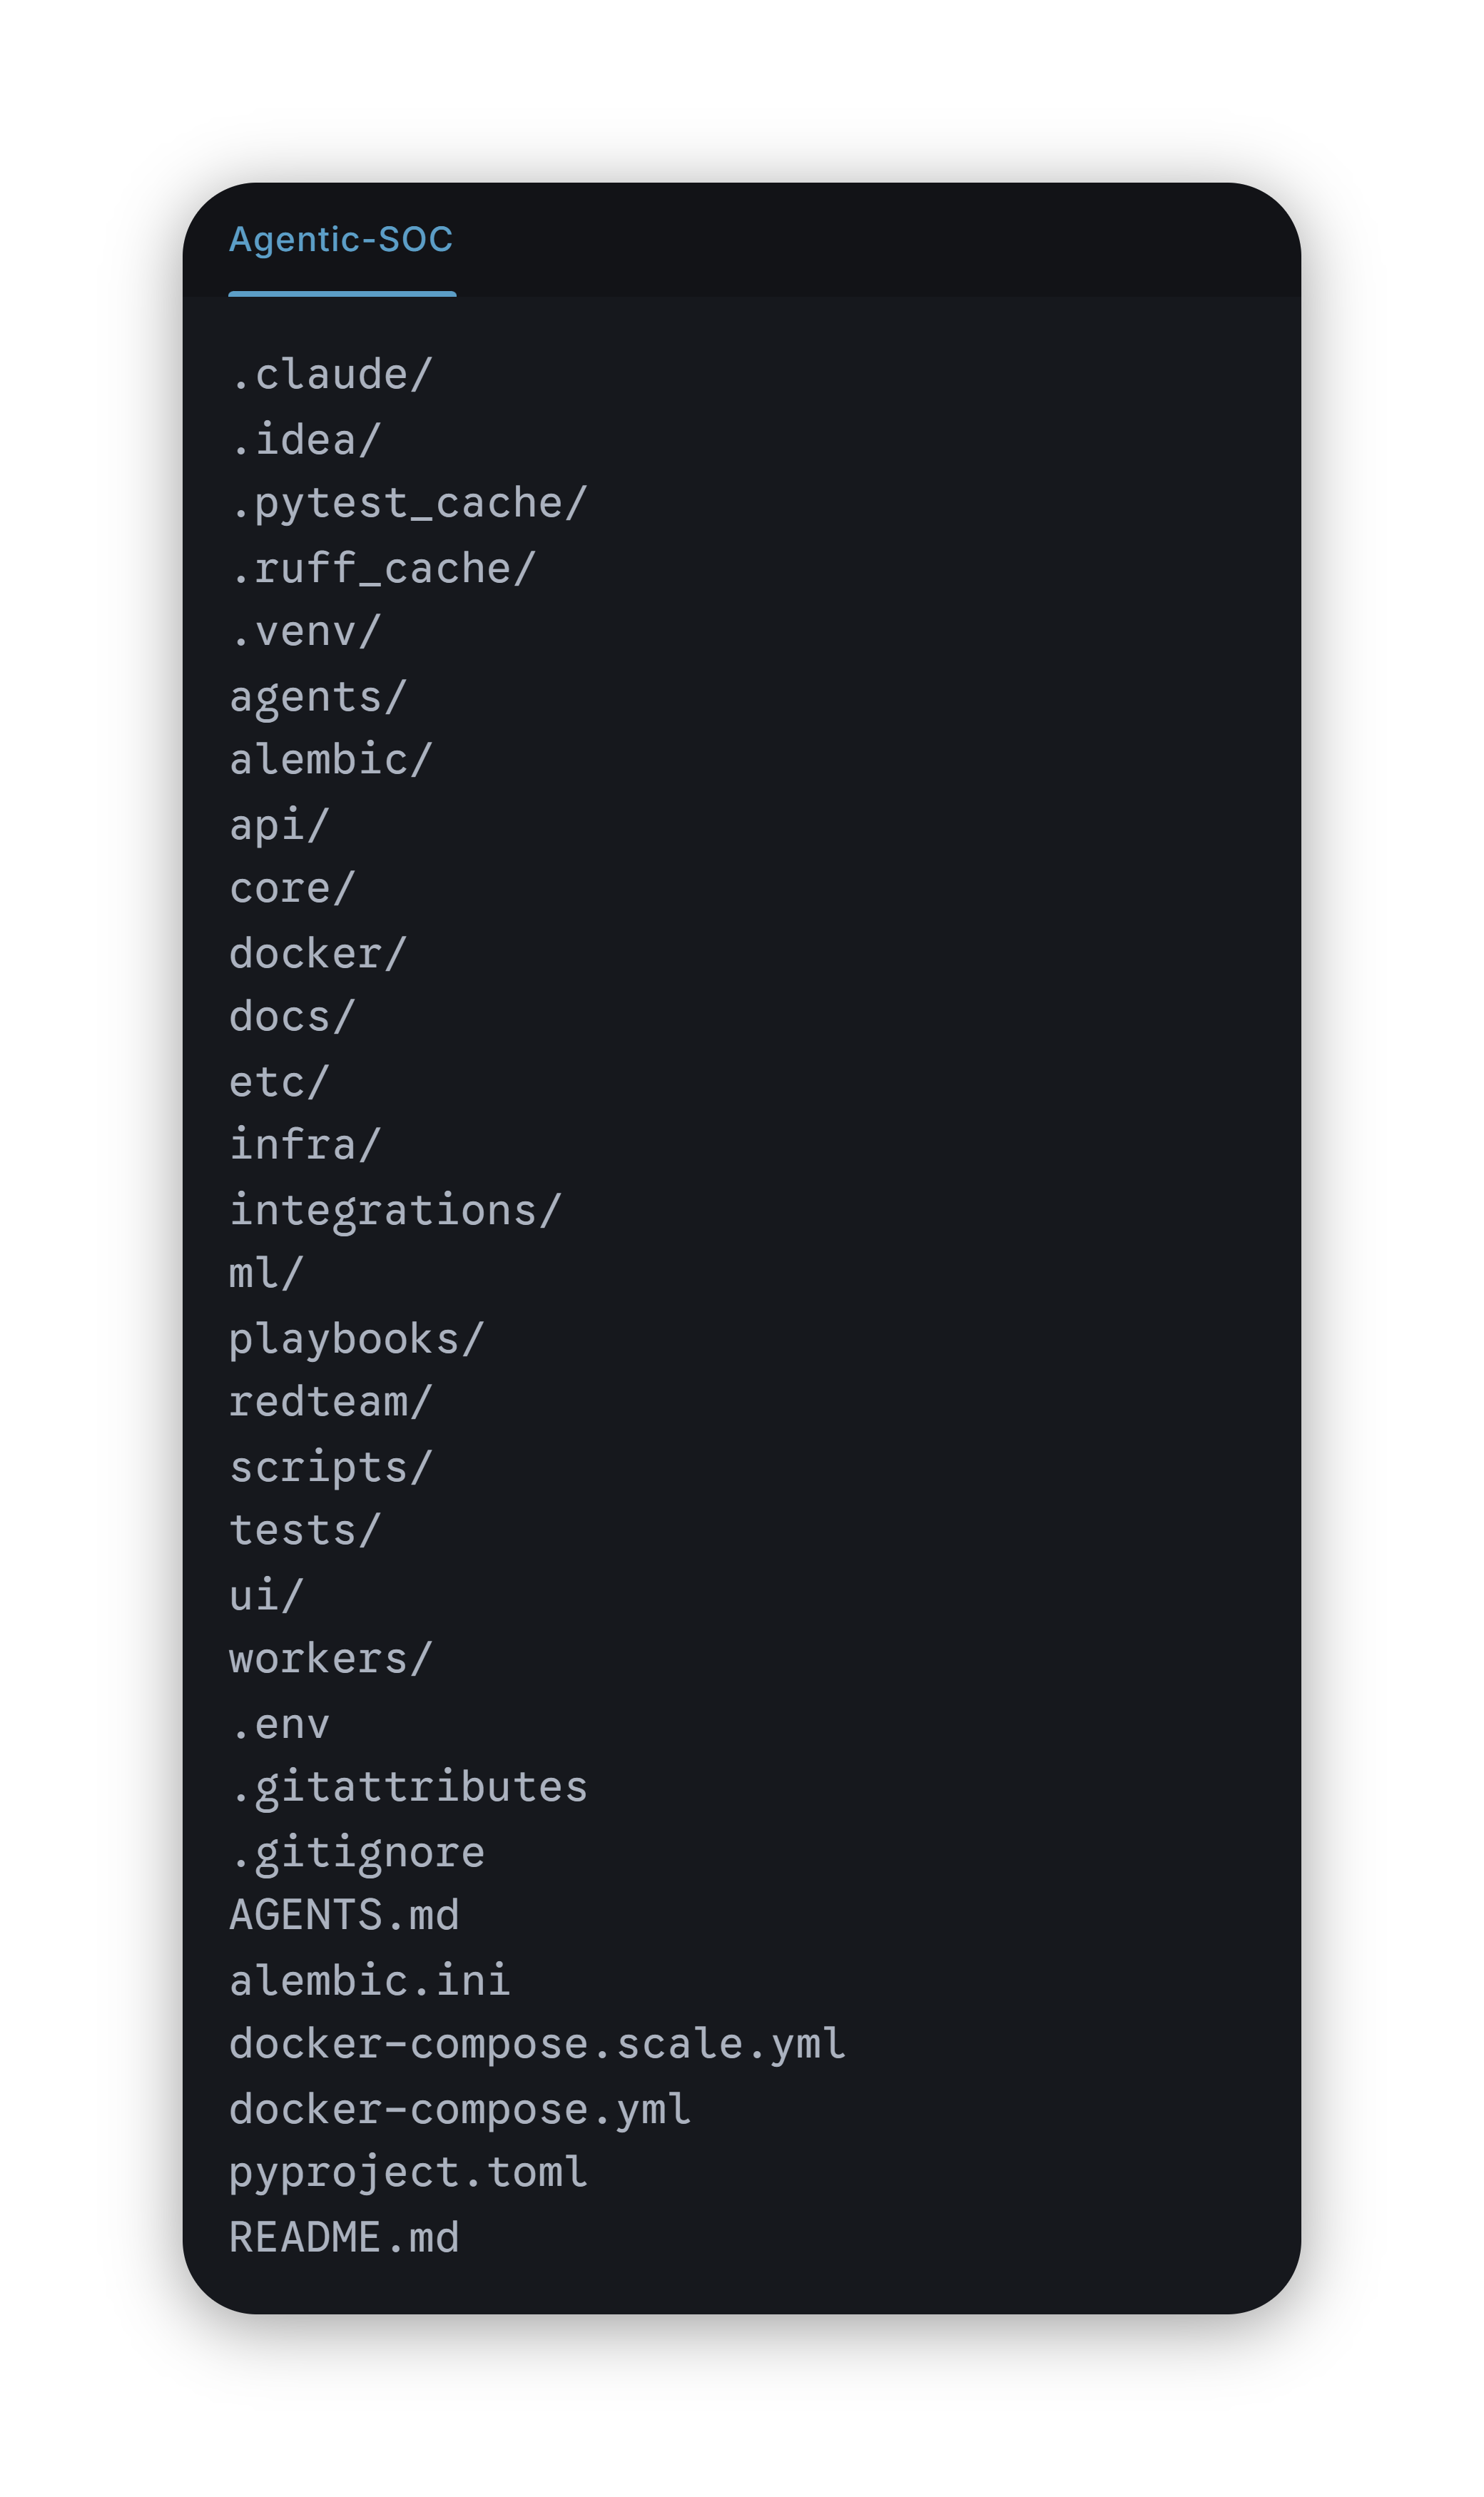
\includegraphics[width=0.75\textwidth]{images/Agentic-SOC_monorepo}
    \caption{Структура монорепозитория}
    \label{fig:monorepo_structure}
\end{figure}

\section{Определение команд, групп и разрешений}

Для обеспечения безопасности разрабатываемого проекта была реализована ролевая модель управления доступом.
Участники практики были разделены на Github Teams, в соответствии с выбранными напрявлениями:

\begin{itemize}
    \item \textbf{RedTeam} --- специалисты по наступательной безопасности --- разработка векторов атак;
    \item \textbf{Engineering} --- инфраструктурные инженеры --- развертывание стендов и их настройка;
    \item \textbf{Dev} --- разработчики --- разработка и поддержка кода системы;
    \item \textbf{Analytics} --- аналитики --- анализ данных и разработка сценариев реагирования;
    \item \textbf{Research} --- исследователи --- изучение технологий и подготовка документации.
\end{itemize}

Командам были выданы права уровня \code{Write} на репозиторий.
Был регламентирован строгий процесс работы с кодом: прямая запись в ветку \code{main} запрещена, все изменения осуществляются через создание новой ветки и последующее открытие Pull Request.
Слияние кода в основную ветку осуществляется только после прохождения Code Review.

\section{Настройка рабочего процесса и инструментов трекинга задач}

Для реализации методологии Agile и визуализации прогресса была создана Канбан-доска с использованием инструмента GitHub Projects.

Процесс отслеживания задач был автоматизирован с помощью следующих механизмов:

\begin{itemize}
    \item \textbf{Labels:} Разработана система меток для классификации задач по треку и типу.
    Например, метки \code{track: Разработка} и \code{type: feature} позволяют быстро идентифицировать задачи, связанные с разработкой новых функций.
    \item \textbf{Milestones:} Проектный план декомпозирован на две ключевые вехи.
    В первой вехе («Испытательный полигон») сгруппированы задачи по развёртыванию инфраструктуры и подготовке стендов.
    Вторая веха («Конвейер тестирования прототипа») включает задачи по интеграции компонентов системы и скриптов автоматизации атак.
    \item \textbf{Automation:} Настроены автоматические действия, такие как автоматическое закрытие задач на доске при слиянии Pull Request.
    Использование ключевых слов, например, \code{Closes \#<номер задачи>} в описании Pull Request позволяет автоматически закрыть задачу и переместить карточку в колонку «Done» на доске.
\end{itemize}

\begin{figure}[H]
    \centering
    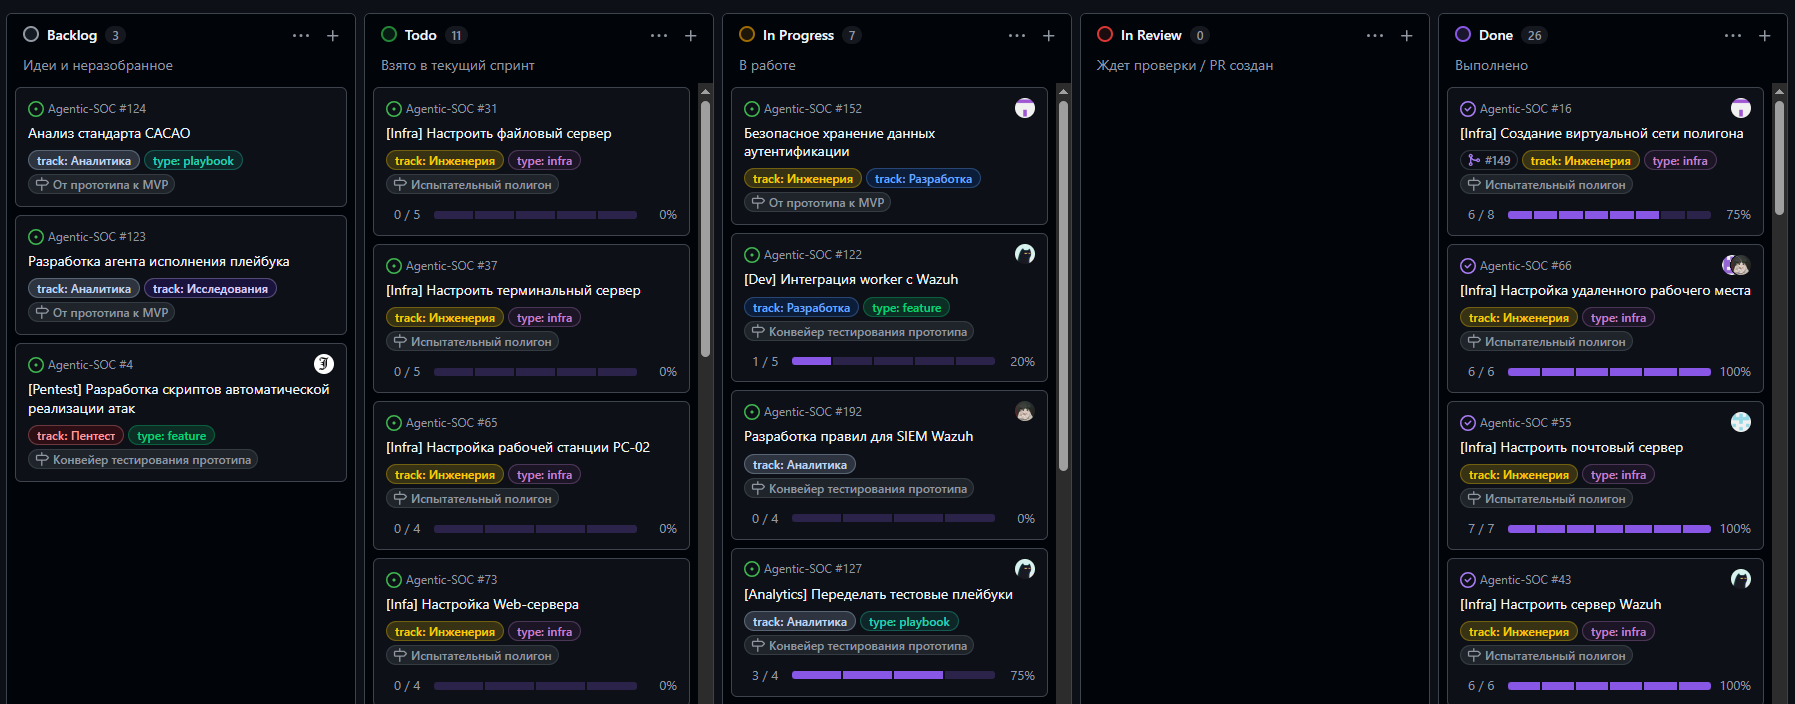
\includegraphics[width=0.8\textwidth]{images/Agentic-SOC_kanban}
    \caption{Канбан-доска проекта}
    \label{fig:kanban_board}
\end{figure}

Реализация первого этапа позволила создать централизованную, отказоустойчивую, прозрачную и масштабируемую среду для совместной работы, соответствующую современным практикам DevSecOps.